\documentclass[letterpaper,11pt]{article}

% Soporte para los acentos.
\usepackage[utf8]{inputenc}
\usepackage[T1]{fontenc}
% Idioma español.
\usepackage[spanish,mexico, es-tabla]{babel}
% Soporte de símbolos adicionales (matemáticas)
\usepackage{multirow}
\usepackage{amsmath}
\usepackage{amssymb}
\usepackage{amsthm}
\usepackage{amsfonts}
\usepackage{mathtools}
\usepackage{latexsym}
\usepackage{enumerate}
\usepackage{listings}
\usepackage[dvipsnames]{xcolor}
\usepackage{float}
\usepackage{graphicx}
\usepackage[linguistics]{forest}

% Modificamos los márgenes del documento.                                       
\usepackage[lmargin=1.5cm,rmargin=1.5cm,top=1.5cm,bottom=1.5cm]{geometry}

\title{Facultad de Ciencias, UNAM \\ 
       Análisis de Algoritmos \\ 
       Tarea 4}
\author{Rubí Rojas Tania Michelle}
\date{26 de enero de 2021}

\begin{document}
\maketitle

\begin{enumerate}
    % Ejercicio 1.
    \item \textit{Mei Hua Zhuang} es una técnica de entrenamiento de Kung Fu, 
    que consiste en $n$ postes grandes parcialmente hundidos en el suelo, con 
    cada poste $p_i$ en la posición $(x_i, y_i)$. Los estudiantes practican 
    técnicas de artes marciales pasando de la parte superior de un poste a la 
    parte superior de otro poste. Pero para mantener el equilibrio, cada paso 
    debe tener más de $d$ metros pero menos de $2d$ metros. Diseñe un algoritmo 
    eficiente para encontrar si es que existe una ruta segura desde el poste 
    $p_s$ al poste $p_t$.

    \textsc{Solución:} Representamos el conjunto de postes como una gráfica 
    $G = (V, E)$. Cada uno de los vértices de $G$ corresponderán a un poste 
    $p_i$ (cuyas coordenadas son $(x_i,y_i)$). Por otro lado, las aristas 
    corresponderán a la adyacencia entre los postes que están en el suelo y 
    tendrán un peso $w_d$ de acuerdo a la distancia (en metros) entre un 
    poste y otro. 

    Si realizamos una búsqueda BFS desde el vértice $p_s$ y en algún momento 
    del recorrido descubrimos el vértice $p_t$, entonces existe un camino entre 
    $p_s$ y $p_t$. Realizándo una modificación para que el camino cumpla con 
    la restricción de la distancia entre los postes, podemos traducir el 
    procedimiento en el siguiente algoritmo:
    \begin{itemize}
        \item Creamos una cola $Q$.
        \item Agregamos el vértice $p_s$ a la cola $Q$.
        \item Marcamos a $p_s$ como visitado.
        \item Mientras $Q$ no esté vacío:
        \begin{itemize}
            \item Sacamos un elemento de la cola $Q$, digamos $v$.
            \item Para cada vértice $w$ adyacente a $v$ en $G$:
            \begin{itemize}
                \item Si el peso (distancia) entre $w$ y $v$ es mayor que $d$ 
                pero menor que $2d$, entonces:
                \begin{itemize}
                    \item Si $w$ es igual a $p_t$, entonces regresamos 
                    \texttt{"Sí existe un camino"}.

                    \item En otro caso, si $w$ no ha sido visitado, entonces 
                    lo marcamos como visitado y lo agregamos dentro de la 
                    cola $Q$.
                \end{itemize}

                \item En otro caso, si $w$ no ha sido visitado, entonces lo 
                marcamos como visitado.
            \end{itemize}
        \end{itemize}

        \item Regresamos \texttt{"No existe un camino"}
    \end{itemize}

    Este algoritmo funciona porque en cada iteración nos aseguramos de seguir 
    un camino donde el peso entre los vértices se encuentra en un rango de 
    $(d, 2d)$; y esto lo logramos gracias al recorrido BFS y una pequeña 
    condición (el de los pesos) para saber cuáles vertices tomar en cuenta y 
    cuáles no. Luego, como el único algoritmo que aplicamos es BFS (modificado 
    por una condición), entonces la complejidad total del algoritmo es 
    $O(V+E)$.
    
    % Ejercicio 2.
    \item El presidente de un país cree que cada ciudad debe de tener acceso 
    a una biblioteca, desafortunadamente el país se vio afectado por un temblor
    que destruyó todas las bibliotecas y bloqueó todos los caminos que había. 
    Dadas $n$ ciudades numeradas de $1$ a $n$, con $m$ caminos bidireccionales, 
    se dice que una ciudad puede acceder a una biblioteca si tiene una construida
    o puede trasladarse a otra ciudad que contenga una. Considerando que los 
    costos de reparación de un camino o de construcción de biblioteca son 
    \texttt{Costo}$_c$ y \texttt{Costo}$_b$, respectivamente. Diseña un algoritmo 
    de tiempo $O(n + m)$ que determine qué caminos reparar y qué bibliotecas 
    construir tal que cada ciudad pueda acceder a una biblioteca y el costo sea 
    mínimo. Por ejemplo, si el \texttt{Costo}$_c \leq$ \texttt{Costo}$_b$, pues 
    la solución es construir a cada ciudad su biblioteca.

    \textsc{Solución:} Representamos al país como una gráfica $G = (V, E)$. 
    Cada uno de los vértices de $G$ corresponderán a una ciudad y las aristas 
    corresponderán a los caminos bidireccionales que existen entre las ciudades.

    % Ejercicio 3.
    \item La \textsc{onu} quiere mandar al espacio dos personas a la luna de
    países distintos. Dada una lista de pares $(i, j)$ donde el $i-$ésimo 
    astronauta es del mismo país que el $j-$ésimo, determina el número de 
    pares posibles a formar. 

    \textsc{Solución:}

    % Ejercicio 4.
    \item Supongamos que tenemos un conjunto de $n$ ciudades $c_1, c_2, \ldots,
    c_n$, y una tabla $D[1 \ldots n,  \ldots n]$ tal que $D[i,j]$ es la longitud 
    de una carretera que une a la ciudad $c_i$ con la ciudad $c_j$ (este valor 
    puede ser $\infty$ si no hay carretera entre $c_i$ y $c_j$). Encuentre un 
    algoritmo eficiente que encuentre la ruta más corta entre las ciudades $c_1$
    y $c_n$ tal que dicha ruta no pasa por más de $k$ ciudades distintas a 
    $c_1$ y $c_n$.

    % Ejercicio 5.
    \item Diseña un algoritmo de tiempo $O(V)$ que determine si una gráfica 
    dirigida $G = (V, E)$ contiene o no un ciclo.

    \textsc{Solución:} Sea $G$ una gráfica con un conjunto de vértices $V(G)$ y 
    un conjunto de aristas $E(G)$. Dado el número de aristas, tenemos dos casos:
    \begin{itemize}
        \item Si el número de aristas de $G$ es menor que $|V(G)|$ entonces puede 
        que tengamos o no un ciclo (pues se requiere que al menos existan tantas
        aristas como vértices para que necesariamente exista un ciclo). Para 
        comprobar esto, recorremos la gráfica usando DFS: si durante el recorrido
        nos encontramos con una arista $e$ que tiene un vértice visitado entonces
        hemos encontrado un ciclo, en caso contrario, no existe algún ciclo. 

        \item Si el número de aristas de $G$ es mayor o igual que $|V(G)|$
        entonces necesariamente tenemos un ciclo.
        \begin{proof}
            Sea $k$ el número de componentes conexas de la gráfica $G$. 
            Realizamos la inducción sobre $k$.
            \begin{itemize}
                \item \textcolor{blue}{Caso base:} $k=1$. Esto quiere decir que 
                $G$ es una gráfica conexa. Como $|E(G)| \geq |V(G)|$, entonces 
                $G$ no puede ser un árbol (pues debería de tener $|V(G)|-1$ 
                aristas), lo que implica que contiene un ciclo.
                
                \item \textcolor{blue}{Hipótesis de inducción.} Supongamos que 
                se cumple para $k$, es decir, supongamos que si el número de 
                aristas de $G$ es mayor o igual que $|V(G)|$ entonces $G$ tiene 
                un ciclo.

                \item \textcolor{blue}{Paso inductivo.}
            \end{itemize}

        \end{proof}

        De esta forma, podemos afirmar que si esta hipótesis se cumple, entonces 
        $G$ tiene un ciclo. En particular, si quisiéramos saber cuál es éste, 
        podemos hacer lo siguiente:
        \begin{itemize}
            \item Si $G$ es conexa, entonces recorremos la gráfica usando DFS
            (iniciándo en un vértice arbitrario). Como la gráfica es conexa, 
            el árbol DFS resultante tendrá todos los vértices de la gráfica, y
            como un árbol tiene $|V(G)|-1$ aristas, entonces existirá al menos una 
            arista en $G$ que no está en el árbol DFS de $G$ (pues 
            $|E(G)| \geq |V(G)|$). Esta arista da un ciclo en $G$.

            \item Si $G$ es disconexa, entonces sabemos que alguna de sus $k$ 
            componentes conexas tiene un ciclo. Bastará con usar la idea del 
            inciso anterior para las componentes conexas para conocer nuestro 
            ciclo.
        \end{itemize}
    \end{itemize}

    Por otro lado, la complejidad del algoritmo efectivamente es $O(V)$. 
    Recordemos que DFS nos toma $O(V + E)$ en tiempo. En el primer caso, como 
    $|E(G)| < |V(G)|$, entonces DFS nos toma $O(V + E) = O(V)$ en tiempo. En 
    el segundo caso, no es necesario buscar el ciclo (pues sólo nos piden una 
    respuesta binaria) ya que sabemos que éste existe. 

    % Ejercicio 6.
    \item Supongamos que tenemos un flujo óptimo en una red $N$ con $n$ vértices,
    (con capacidades enteras) de un nodo fuerte $s$ a un nodo destino $t$.
    \begin{itemize}
        % Ejercicio 6.a
        \item Supongamos que la capacidad de una sola arista $e$ se incrementa 
        en una unidad. De un algoritmo de tiempo $O(n + E)$ para actualizar
        nuestro flujo. $E$ es el número de aristas de $N$.

        \textsc{Solución}: Sabemos que este incremento no puede disminuir el 
        flujo máximo de la red $N$, pues todo flujo de la red original es un 
        flujo de la red modificada. Además, si existe un corte mínimo en el que 
        $e$ no se encuentra, entonces el flujo máximo no se puede incrementar, 
        por lo que no existirá ningún camino aumentante en la red residual.

        % Ejercicio 6.b
        \item Supongamos que la capacidad de una sola arista $e$ se decrementa
        en una unidad. De un algoritmo de tiempo $O(n + E)$ donde $E$ es el 
        número de aristas de $N$.

        \textsc{Solución:}
    \end{itemize}

    % Ejercicio 7.
    \item El profesor Protón tiene dos hijos, los cuales no se llevan nada 
    bien. Los chiquillos se odian tanto que no sólo se niegan a caminar juntos
    a la escuela, sino que además se niegan a caminar en cualquier acera en la 
    que el otro hermano haya puesto un pie ese día. Los chiquillos no tienen 
    problema con que sus caminos coincidan en algunas esquinas. Afortunadamente,
    tanto la cada del profesor como la escuela están en una esquina, fuera de 
    eso, el profesor no está seguro si será posible meter a los dos hijos en 
    la misma escuela. Muestre cómo modelar el problema de decidir si es posible 
    enviar a los dos hijos a la misma escuela como un problema de flujos.
    
    \textsc{Solución:} Representamos el mapa del pueblo del profesor Protón como 
    una gráfica dirigida $G = (V, E)$, donde los vértices de $G$ serán las 
    esquinas y existirá una arista entre dos vértices en caso de que haya una 
    banqueta que las une (creamos una arista también en la dirección contraria 
    como lo hicimos en clase para los problemas de flujos). Después, definimos 
    la capacidad de flujo de cada arista de la red de flujos como $c(u,v) = 1$, 
    pues los chiquillos no quieren pisar la misma banqueta que su hermano. El
    nodo fuente $s$ será la casa del profesor Protón, mientras que el nodo 
    destino $t$ será la escuela (ambos puntos del mapa son vértices ya que se 
    encuentran en esquinas). 

    El flujo de una arista $f(u,v)$ será de una unidad en caso de que un niño
    vaya por la banqueta que une las esquinas $u, v$. Por la restricción de 
    capacidad $0 \leq f(u,v) \leq c(u,v)$, entonces estamos modelándo 
    correctamente el hecho de que los chiquillos no usen la misma banqueta. 
    Si existieran dos caminos distintos de la casa del profesor Protón a la 
    escuela, entonces el flujo de la red tendría que ser mayor o igual a $2$, ya 
    que sería posible asignar un flujo de una unidad ($f(u,v) = 1$) para cada 
    arista. Por otro lado, si sólo existiera un camino distinto de la casa a 
    la escuela, entonces esto implicaría que existe un puente, digamos la arista
    $(x,y)$, que al eliminarla dejaría desconectada a la casa de la escuela. 
    Al haber definido la capacidad de cada arista de una unidad, entonces en 
    particular tenemos que $c(x,y) = 1$ y así el máximo flujo que puede llegar
    al vértice $x$ sería de una unidad. Luego, por la conservación de flujos, 
    tenemos que el flujo desde la casa hasta el vértice $y$ puede ser a lo más 
    de una unidad, es decir, 
    \begin{equation*}
        f = \sum_{v \in V} f(s, y) \leq 1
    \end{equation*}

    Por consecuente, tenemos que el hecho de determinar el flujo máximo y ver 
    que éste sea mayor o igual a $2$ le servirá al profesor para poder 
    averiguar si puede llevar a los chiquillos a la misma escuela o no.

    Ahora bien, el algoritmo que resuelve el problema de encontrar el flujo 
    máximo en una red de flujos (gráficas dirigidas y acíclicas) es el de 
    \texttt{Ford-Fulkerson}, cuyo método general está basado en los caminos 
    aumentantes:
    \begin{figure}[H]
        \centering
        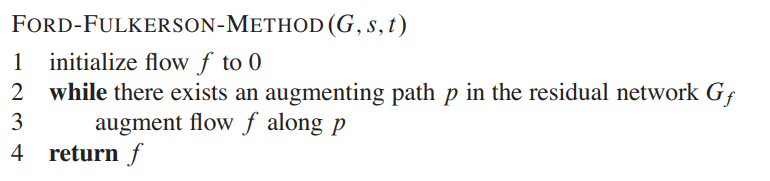
\includegraphics[width=0.5\textwidth]{imagenes/FORD.png}
        \caption{Cormen, Introduction To Algorithms pag. 715}
    \end{figure}

    En donde la red residual mencionada es de manera intuitiva aquella que 
    consiste de las aristas con capacidades que representan cómo han 
    cambiado los flujos de las aristas de la gráfica $G$ y un flujo $f$. 
    De manera formal, la capacidad residual en una red de flujos $G = (V, E)$
    con origen $s$ y destino $t$, un flujo $f$ en $G$ y un par de vértices 
    $u,v \in G$ se define de la siguiente forma:
    \begin{equation*}
        c_f(u,v) = 
        \begin{cases}
            c(u,v) - f(u,v) & (u,v) \in E \\ 
            f(u,v) & (v,u) \in E \\ 
            0 & \text{otherwise}
        \end{cases}
    \end{equation*}

    Y así la red residual de $G$ inducida por el flujo $f$ será $G_f(V, E_f)$ 
    donde
    \begin{equation*}
        E_f = \{(u,v) \in V \times V \; | \; c_f(u,v) > 0\}
    \end{equation*} 

    Que es lo que hacíamos en clase al ir actualizándo el flujo de una arista, 
    luego reduciéndo su capacidad y poniéndo el flujo restante en el otro 
    sentido.

    Finalmente, un pseudocódigo de la implementación de la técnica de 
    \texttt{Ford-Fulkerson} sería el siguiente:
    \begin{figure}[H]
        \centering
        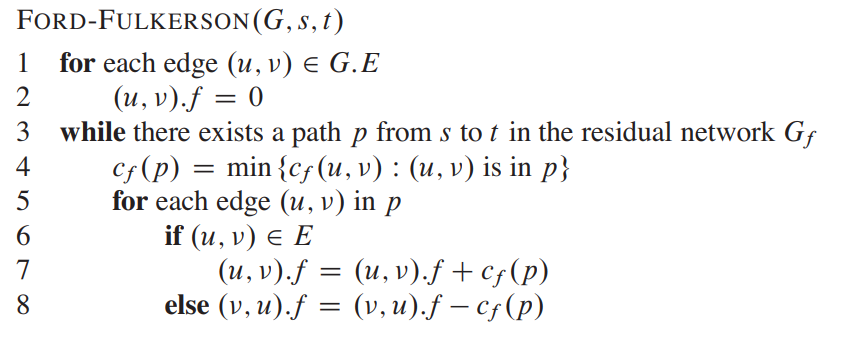
\includegraphics[width=0.5\textwidth]{imagenes/pseudo.png}
        \caption{Cormen, Introduction To Algorithms pag. 724}
    \end{figure}

    Como lo indica el \texttt{Cormen}, la complejidad de la implementación 
    dependerá de la línea $3$ (donde se buscan los caminos aumentantes).
    Si se emplean búsquedas BFS o DFS, entonces cada iteración de la línea 
    $3$ usará tiempo $O(E)$, al igual que la inicialización de las líneas 
    $1-2$. Luego, como el ciclo que corresponde a las líneas $4-8$ se 
    ejecuta a lo más $|f^*|$ veces, donde $f^*$ denota el flujo máximo en 
    la red de flujos transformada, pues en cada iteración el flujo se ve 
    incrementado al menos en una unidad. Así, la complejidad de todo el 
    algoritmo sería de $O(E|f^*|)$ tiempo.

    % Ejercicio 8.
    \item It is a natural to apply graph models and algorithms to spatial 
    problems. Consider a black and white digitalized image of a maze; white 
    pixels represents open areas and black spaces are walls. There are two
    spacial white pixels: one is designated the entrance and the other is the 
    exit. The goal in this problem is to find a way of getting from the entrance 
    to the exit, as ilustrated in Figure $1$. Given a $2D$ array of black and 
    white entries representing a maze with designated entrance and exit points, 
    find a path from the entrance to the exit, if one exists.
    \begin{figure}[H]
        \centering
        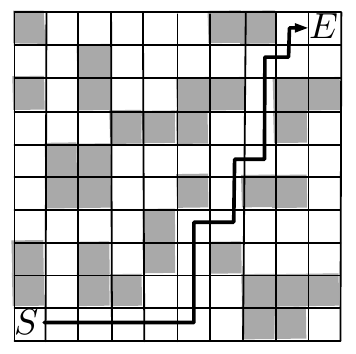
\includegraphics[width=0.21\textwidth]{imagenes/path.png}
        \caption{A shortest path from entrance to exit.}
    \end{figure}

    \textsc{Solución:} Representamos el laberinto como una gráfica $G = (V, E)$.
    Cada uno de los vértices de $G$ corresponderán a un píxel blanco (zona 
    abierta) y estarán indexados de acuerdo a sus respectivas posiciones en la 
    matriz $2D$ (es decir, el vértice $v_{i,j}$ corresponde al píxel blanco en 
    la entrada $(i,j)$ del arreglo $2D$). Por otro lado, las aristas 
    corresponderán a la adyacencia entre los píxeles blancos (es decir, dos
    píxeles blancos que sean adyacentes en la matriz $2D$ estarán unidos por
    una arista en la gráfica $G$).

    Sea $p_i$ y $p_f$ la entrada y salida del laberinto, respectivamente. 
    Si realizamos una búsqueda BFS desde el vértice $p_i$ y en algún momento 
    del recorrido descubrimos el vértice $p_f$, entonces existe un camino entre 
    $p_i$ y $p_f$. Para encontrar dicho camino, basta con ir guardando cada uno 
    de los vértices que lo van formando en una lista. De esta manera, podemos 
    traducir este procedimiento en el 
    siguiente algoritmo:
    \begin{itemize}
        \item Creamos una cola $Q$ y una lista $P$.
        \item Agregamos $p_i$ a la cola $Q$.
        \item Marcamos $p_i$ como visitado.
        \item Mientras $Q$ no esté vacío:
        \begin{itemize}
            \item Sacamos un elemento de la pila $Q$, digamos $v$.
            \item Agregamos a $v$ a la lista $P$.
            \item Para cada vértice $w$ adyacente a $v$ en $G$:
            \begin{itemize}
                \item Si $w$ es igual a $p_f$, entonces agregamos $p_f$ a la 
                lista $P$ y regresamos esta lista. Terminamos.
                \item En otro caso, si $w$ no ha sido visitado, entonces 
                marcamos como visitado a $w$ e insertamos $w$ dentro de la 
                cola $Q$.
            \end{itemize}
        \end{itemize}

        \item Regresamos la lista vacía (pues no encontramos un camino).
    \end{itemize}

    Este algoritmo funciona debido a que en cada iteración garantizamos tener
    los vértices que pertenecen al camino entre $p_i$ y $p_f$ (si es que 
    existe) al utilizar BFS para recorrer la gráfica $G$ y en el transcurso ir 
    guardándo los vértices del camino que vamos recorriéndo en una lista $P$. 
    Además, BFS encuentra el camino más corto: como exploramos todos los hijos
    inmediatos antes de pasar a los nietos, entonces garantiza que todos los 
    nodos a una distancia determinada del nodo padre se exploren al mismo tiempo.

    Ahora bien, sabemos que la complejidad de BFS es $O(V+E)$ y como las únicas 
    operaciones extra que realizamos son la creación de una lista $P$ e ir 
    agregando elementos a ella (ambas en tiempo constante), entonces la 
    complejidad total del algoritmo es de $O(V + E)$.
\end{enumerate}

\end{document}
